\chapter{Results}



This chapter discusses the results obtained when testing both the Complementary Filter and Kalman Filter. Initially the pitch angles were plotted over time with different \gls{noisecoplantmatrix} values until the best results was obtained. The estimated orientation from the Complementary Filter, Kalman Filter and the potentiometer data were plotted on the same graphs and compared.

\section{The Complementary Filter}
\subsection{The effect $\tau$ on Estimation}
The effect of $\tau$ on the estimate was tested by varying $\tau$ and can be seen in Figure \ref{fig effect of tau on filter}. Figure \ref{fig effect of tau on filter} compares the estimated data from the Complementary Filter with the actual values from the potentiometers. As seen in Figure \ref{fig effect of tau on filter} of the value of $\tau$ is set too low the accelerometer becomes the driving factor and the estimate remains noisy. While if $\tau$ is set too high the gyroscope data is used more than the accelerometer, hence a delay is introduced. Thus, a middle ground which will give an adequate estimate of the attitude of the quad-rotor. The best choice of $\tau$ was found to be 0.468 for use with this system. 


\begin{figure}[h]
	\centering
	\begin{subfigure}{0.32\textwidth}
		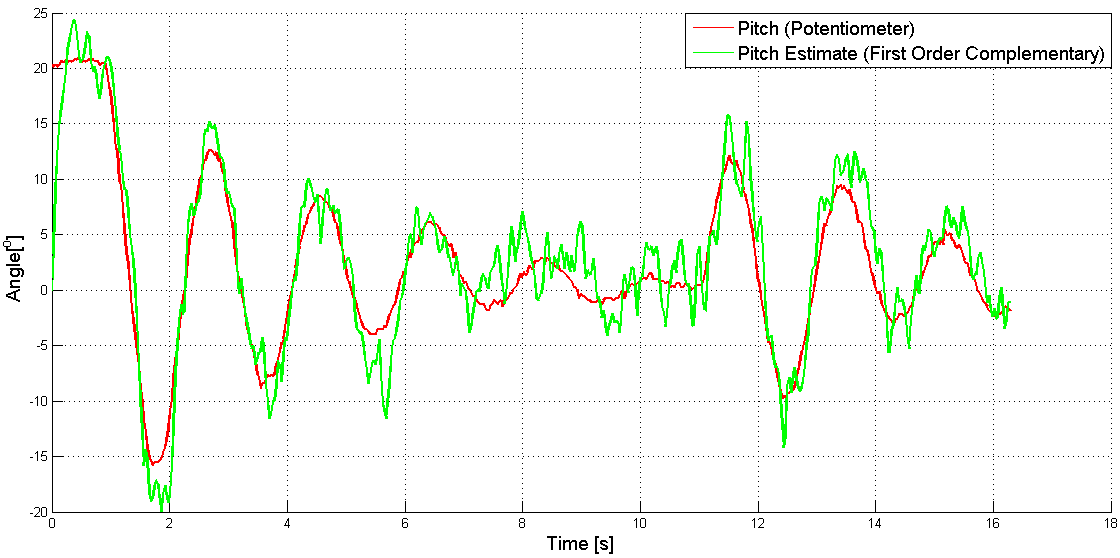
\includegraphics[width =0.38\paperwidth]{\DocRoot/images/comp_first_order_low}
		\caption{Pitch estimate with $\tau$ = 0.1}
		\label{Fig:low tau}
	\end{subfigure}%
	\hspace{3cm}
	\begin{subfigure}{0.32\textwidth}
		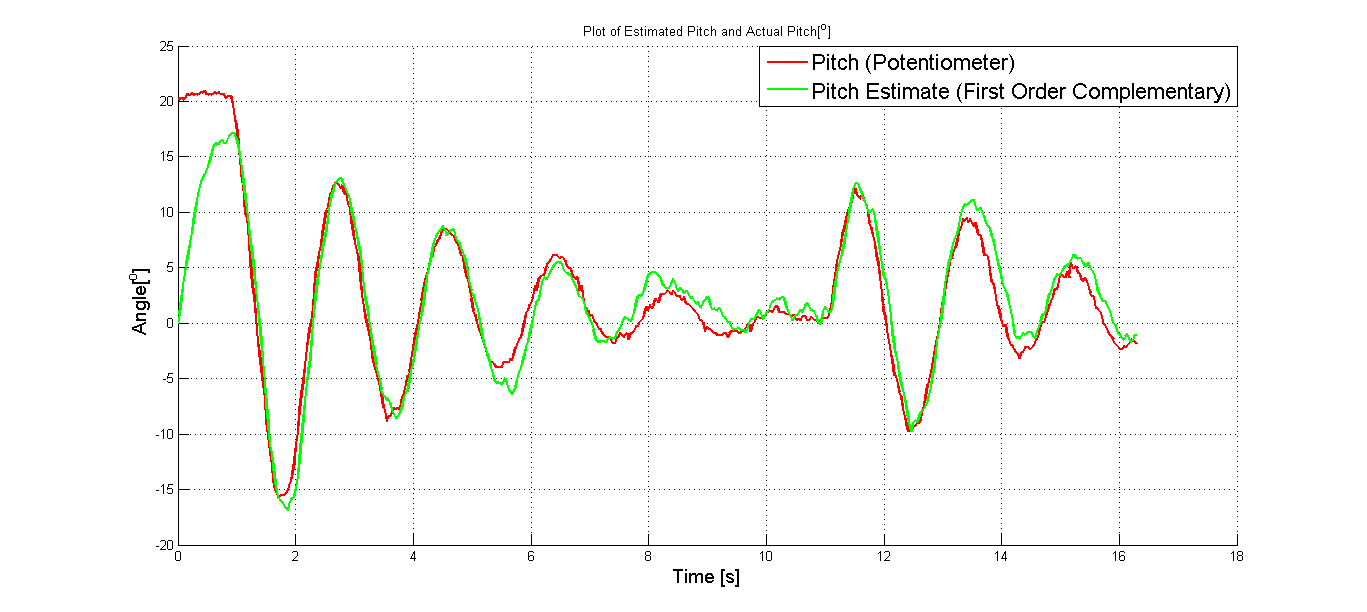
\includegraphics[width =0.38\paperwidth]{\DocRoot/images/comp_first_order_time}
		\caption{Pitch estimate with $\tau$ = 0.5}
		\label{Fig:high tau}
	\end{subfigure}
	\caption{Effect of varying $\tau$ on the estimate produced by the Complementary Filter}	
	\label{fig effect of tau on filter}
\end{figure}


\section{The Kalman Filter}
\subsection{Effect of Q on Estimation} 
The effect \gls{noisecoplantmatrix} has on the estimated was tested by varying the \gls{noisecoplantmatrix} matrix and comparing the estimated data from the Kalman Filter with the actual values from the potentiometers. In these tests, \gls{noisecomatrix} was kept constant at its theoretical value since it is the ratio of the two parameters that effect the estimate.


\begin{figure}[h]
	\centering
	\begin{subfigure}{0.32\textwidth}
		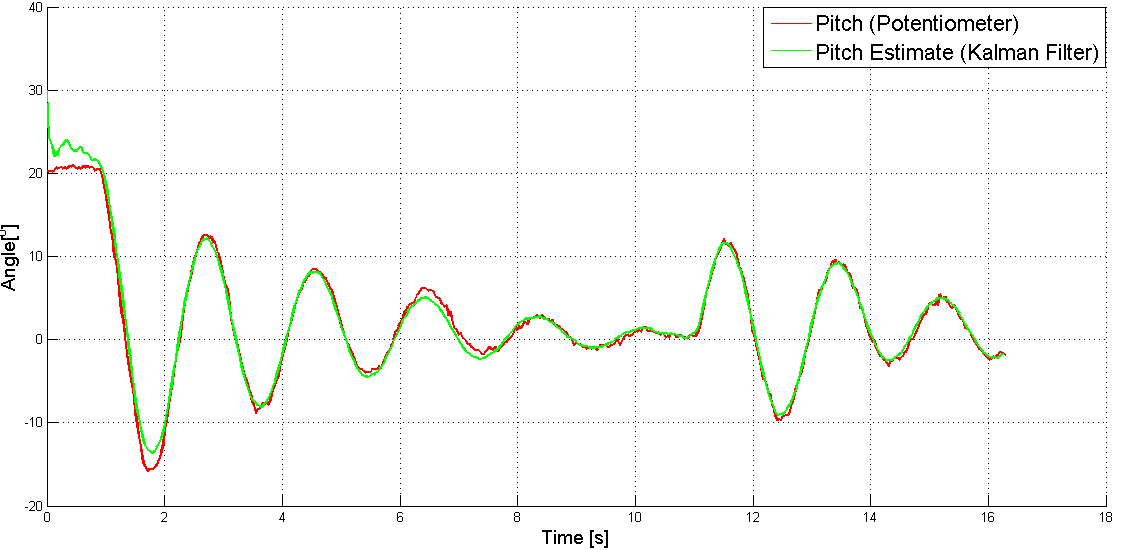
\includegraphics[width =0.38\paperwidth]{\DocRoot/images/Kalman_low}
	\caption{Pitch estimate with \gls{noisecoplantmatrix}/\gls{noisecomatrix} = $8.805\times10^{-5}$}
	\label{Fig:q/r ratio low}
	\end{subfigure}%
	\hspace{3cm}
	\begin{subfigure}{0.32\textwidth}
		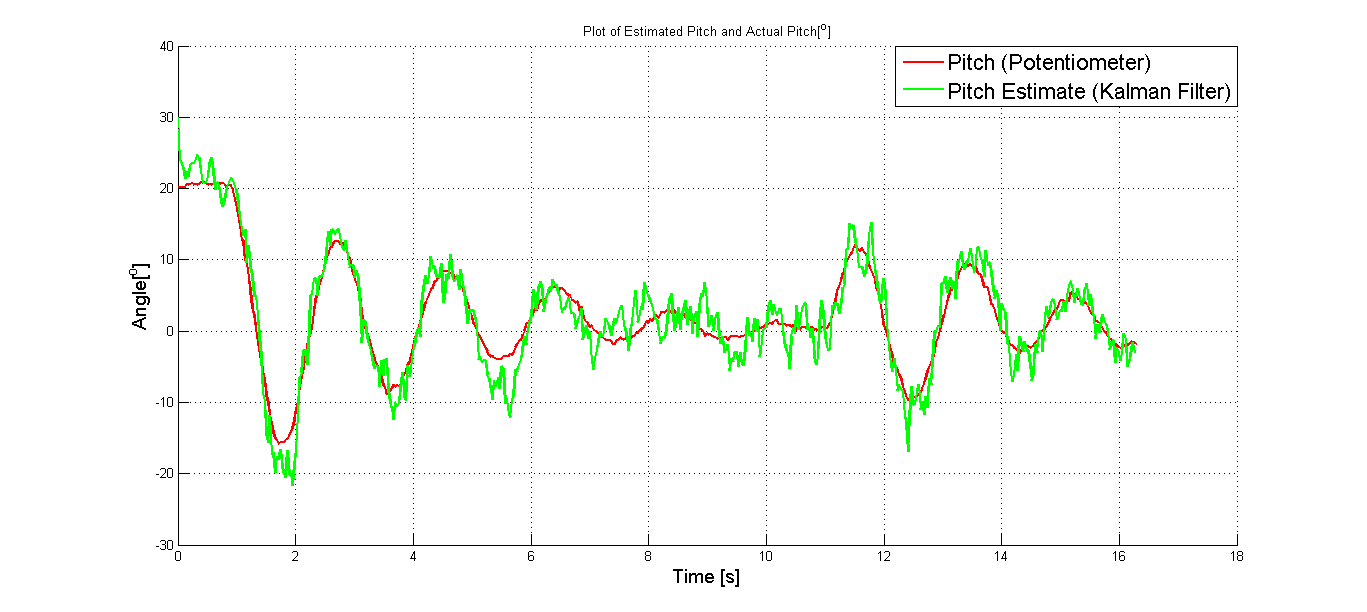
\includegraphics[width =0.38\paperwidth]{\DocRoot/images/Kalman_high}
	\caption{Pitch estimate with \gls{noisecoplantmatrix}/\gls{noisecomatrix} = 0.0881}
	\label{Fig:q/r ratio high}
	\end{subfigure}
	
	\caption{Effect of varying \gls{noisecoplantmatrix}/\gls{noisecomatrix} on the estimate produced by the Kalman Filter }	
\end{figure}
Figure \ref{Fig:q/r ratio low} and \ref{Fig:q/r ratio high} clearly show that the estimate of the pitch angles varies with \gls{noisecoplantmatrix}. At a lower \gls{noisecoplantmatrix} than \gls{noisecomatrix}, the response of the filter is more accurate. This implies that there is less noise on the states relative to the  measured signals. The Kalman Filter in this case assumes that the predicted pitch values are reliable and need little correction. Therefore increasing the Kalman gain matrix places more emphasis on the measurements and less on the prediction values \cite{gordon_paper}

Figure \ref{Fig:Cross-Correlation of estimated pitch error} shows the cross-correlation of the error between the estimated and actual pitch values. If the noise present in the Kalman Filter's model and the present in the accelerometer and gyros is Gaussian and uncorrelated, Figure \ref{Fig:Cross-Correlation of estimated pitch error} would be all zero except at the center, where the response would be one. Therefore, Figure \ref{Fig:Cross-Correlation of estimated pitch error} shows that the noise present in the signals is not uncorrelated.

\begin{figure}[h]
	\centering
	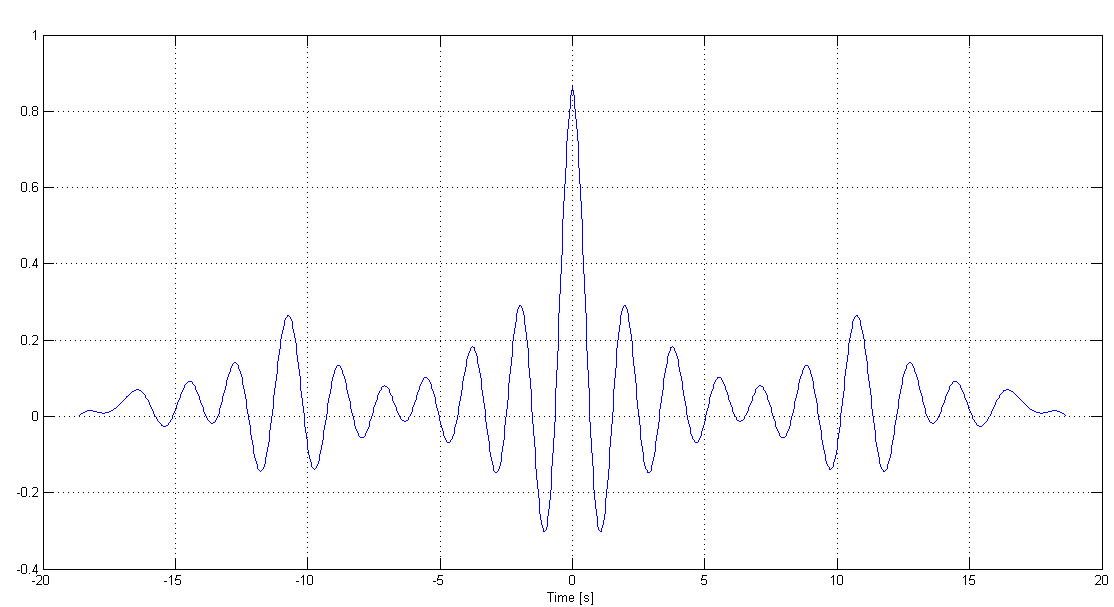
\includegraphics[width =0.8 \paperwidth]{\DocRoot/images/corelation_matlab}
	\caption{Cross-Correlation of estimated pitch error}
	\label{Fig:Cross-Correlation of estimated pitch error}
\end{figure}